%%%%%%%%%%%%%%%%%%%%%%%%%%%%%%%%%%%%%%%%%
% University Assignment Title Page 
% LaTeX Template
% Version 1.0 (27/12/12)
%
% This template has been downloaded from:
% http://www.LaTeXTemplates.com
%
% Original author:
% WikiBooks (http://en.wikibooks.org/wiki/LaTeX/Title_Creation)
%
% License:
% CC BY-NC-SA 3.0 (http://creativecommons.org/licenses/by-nc-sa/3.0/)
% 
% Instructions for using this template:
% This title page is capable of being compiled as is. This is not useful for 
% including it in another document. To do this, you have two options: 
%
% 1) Copy/paste everything between \begin{document} and \end{document} 
% starting at \begin{titlepage} and paste this into another LaTeX file where you 
% want your title page.
% OR
% 2) Remove everything outside the \begin{titlepage} and \end{titlepage} and 
% move this file to the same directory as the LaTeX file you wish to add it to. 
% Then add \input{./title_page_1.tex} to your LaTeX file where you want your
% title page.
%
%%%%%%%%%%%%%%%%%%%%%%%%%%%%%%%%%%%%%%%%%


%----------------------------------------------------------------------------------------
%	PACKAGES AND OTHER DOCUMENT CONFIGURATIONS
%----------------------------------------------------------------------------------------

\documentclass{article}
% Please add the following required packages to your document preamble:
\usepackage{multirow}
\usepackage[normalem]{ulem}
\useunder{\uline}{\ul}{}
\usepackage{textcomp}
\usepackage{afterpage}
\usepackage{cite}
\usepackage{rotating}
\usepackage{booktabs}
\usepackage{float}
\usepackage{amsmath}
\usepackage{mathtools}
\usepackage[toc,page]{appendix}
\usepackage{multicol}
\usepackage[utf8]{inputenc}
\usepackage[]{graphicx}
\usepackage[export]{adjustbox}
\usepackage{multicol}
\usepackage{subcaption}
\usepackage{caption}
\usepackage[font=small,labelfont=bf]{caption}
\usepackage{enumitem}
\setlist{nolistsep}                         % no white line between list items
\newlist{steps}{enumerate}{1}               % step 1, step 2, etc. \begin
\setlist[steps, 1]{label = Step \arabic*:}  % \end
\usepackage{listings}
\usepackage{url}
\usepackage{tabto}
\usepackage{hyperref}
\usepackage{eurosym}
\usepackage[top=2.2cm,bottom=2.2cm,left=2.2cm,right=2.2cm]{geometry}
\setlength{\parindent}{2em}                 % use \par end of paragraph, indent will follow
\usepackage[table,xcdraw]{xcolor}           % color cells in table
\usepackage{siunitx}                        % SI units
\usepackage{adjustbox}                      %rotate boxes in an angle X: \begin{adjustbox}{angle=X}

\usepackage{color} %red, green, blue, yellow, cyan, magenta, black, white
\definecolor{mygreen}{RGB}{28,172,0} % color values Red, Green, Blue
\definecolor{mylilas}{RGB}{170,55,241}

\usepackage{datetime}
\newdateformat{monthyeardate}{%
  \monthname[\THEMONTH], \THEYEAR}
\usepackage{dingbat}
\usepackage{caption}                        %\captionsetup[table]{skip=5pt}
\usepackage{gensymb}
\usepackage{pdfpages}                       % add pdf pages to document
\setlength{\columnsep}{2cm}
\usepackage[normalem]{ulem}
\newcommand{\Tau}{\mathrm{T}}               % add \Tau as option to document
\usepackage{minted}                         % nice python scripts, \begin{minted}[linenos,breaklines]{python}
\usepackage{array}
\usepackage{verbatim}                       % \begin{comment}  [....] \end{comment}
\usepackage[utf8]{inputenc}
\usepackage[T1]{fontenc}
\usepackage{tikz}
\newcommand{\fatterdot}{\raisebox{0.25ex}{\tikz\filldraw[black,x=2pt,y=2pt] (0,0) circle (1);}}
\usepackage{blindtext}
%\usepackage{cleveref}
\usepackage{pgfgantt}
\usepackage{xcolor}
\usepackage[utf8]{inputenc}

\newcommand*{\eqautoref}[1]{%
  \begingroup
    \def\equationautorefname{eq.}%
    \autoref{#1}%
  \endgroup
}

\newcommand*{\figautoref}[1]{%
  \begingroup
    \def\equationautorefname{fig.}%
    \autoref{#1}%
  \endgroup
}

\definecolor{barblue}{RGB}{33,87,50}
\definecolor{groupblue}{RGB}{0,87,50}
\definecolor{linkred}{RGB}{33,0,50}
\begin{document}

%Cover page



%Title
\begin{titlepage}

\newcommand{\HRule}{\rule{\linewidth}{0.5mm}} % Defines a new command for the horizontal lines, change thickness here

\center % Center everything on the page
 
%----------------------------------------------------------------------------------------
%	HEADING SECTIONS
%----------------------------------------------------------------------------------------

\textsc{\LARGE Simulation, Verification \& Validation}\\[1cm] % Name of your university/college
\textsc{\Large AE3212-II}\\[0.5cm] % Major heading such as course name
%\textsc{\large Minor Heading}\\[0.5cm] % Minor heading such as course title

%----------------------------------------------------------------------------------------
%	TITLE SECTION
%----------------------------------------------------------------------------------------

\HRule \\[0.4cm]
{ \huge \bfseries Simulation Plan \\ \vspace{3mm} Group A36}\\[0.4cm] % Title of the document
 %SUBTITLE HERE%
\HRule \\[1.5cm]

%----------------------------------------------------------------------------------------
%	AUTHOR SECTION
%----------------------------------------------------------------------------------------


\begin{minipage}{0.3\textwidth}
\begin{flushleft} \large

\emph{Amant, Bram                 \\
        Berger, Menno               \\
        Helsdingen, Wieger          \\
        Hinssen, Yara               \\
        Sirghi, Florina             \\
Wegener, Malte              \\}
\textsc{} % Your name
\end{flushleft}
\end{minipage}
~
\begin{minipage}{0.3\textwidth}
\begin{flushright} \large

\emph{ 
        4672291                    \\
        4667921                     \\
        4547101                     \\
        4659023                     \\
        4648579                     \\
        4672194                     \\}
          
 \textsc{} % Student number
\end{flushright}
\end{minipage}\\[1.5cm]


% If you don't want a supervisor, uncomment the two lines below and remove the section above
%\Large \emph{Author:}\\
%John \textsc{Smith}\\[3cm] % Your name



%----------------------------------------------------------------------------------------
%	DATE SECTION
%----------------------------------------------------------------------------------------
\vfill % Fill the rest of the page with whitespace

{\large \monthyeardate\today}\\ % Date, change the \today to a set date if you want to be precise
\textsc{Version 1.0}\\[0.5cm]

%----------------------------------------------------------------------------------------
%	LOGO SECTION
%----------------------------------------------------------------------------------------

%\includegraphics{Logo}\\[1cm] % Include a department/university logo - this will require the graphicx package

%\textsc{Track Coordinators: } \\
%\textsc{Teaching assistant:}


\vfill % Fill the rest of the page with whitespace
%----------------------------------------------------------------------------------------
\begin{figure}[H]
    \centering
    
\includegraphics[width=0.4\textwidth]{Images/titlepage/tudelft-logo (1).jpg}
    %\caption{Caption}
    \label{coverfigure}
\end{figure}



\end{titlepage}


% Table of contents
\tableofcontents
\newpage

% Content

\pagenumbering{roman}
\newpage
\pagenumbering{arabic}
\newpage
\section{Introduction}
\label{Introduction}

%Problem statement: What are the deflection, twist and maximum stress experienced by the aileron under a critical loading scenario.

An aileron is a control surface of an aircraft, located towards the tip of the wing. It provides maneuverability and stability during different parts of flight. The optimum operation of the aileron is necessary at all times in order to ensure the safety of the passengers, cargo and the crew during flight. Thus, correct functioning of the aileron is required even in a critical loading scenario. The critical loading scenario that is currently analysed consists of the aileron being at maximum upward deflection and the aerodynamic loading on the
wing being at limit load. Furthermore, one of the two actuators of the aileron is jammed. In this case, the aileron is subjected to bending, shear and torsion. \\

\noindent In order to observe the behaviour of the aileron of the Fokker 100 in this critical loading scenario, a numerical structural analysis tool needs to be developed. The tool will have as outputs the deflection of the hinge line, the twist of the aileron, and the maximum stress experienced by the aileron.\\

\noindent This report outlines the simulation plan for the actual implementation, verification and validation of the numerical model. In this report, the description of the loading cases is presented first. Then, the theory behind the numerical model as well as the approach regarding its implementation are described. Next, the verification model is discussed, followed by the verification strategy proposed for the team's own numerical model. After this, the validation approach of the constructed model is discussed. The task division as well as a Gantt chart may be found in the Appendices.   

\newpage
\section{Load Case}
\label{sec:loading}

\textit{The first step of every structural analysis problem is defining the exact problem. To do that free body diagrams are constructed to show geometry, dimensions and acting forces and moments. Then, an accurate and detailed description of the load case is required to ensure realistic results.}

\subsection{Loading scenario}
The concerned loading case of the aileron is caused by the critical loading scenario of the Fokker 100. This scenario is a combination of a couple elements: The aileron is deflected to it's maximum potential upward deflection which is 30 degrees. Also, the aerodynamic loading of the wing is at the limit load. Lastly, one of the actuators used to control the aileron is jammed while the second actuator is giving a discrete load in the negative z-direction.

\subsection{Reference frame}
The reference frame used for the model has its x-axis in span wise direction, pointing towards the tip of the undeformed main wing. The z-axis is in chord wise direction, pointing towards the leading edge. Finally, the y-axis is directed upwards, orthogonal to the aileron surface. This reference frame is visualised in \figautoref{reference_frame}.

\begin{figure}[H]
    \centering
    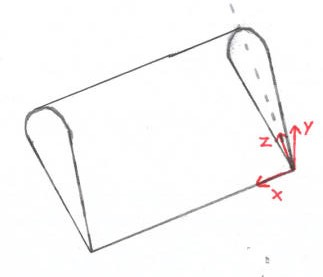
\includegraphics[width=4.5cm]{Images/reference_frame.jpg}
    \caption{Reference frame}
    \label{reference_frame}
\end{figure}


\subsection{Geometry and specifications}
The geometry of the aileron is visualised in \figautoref{fig:Dimensions_top_view}, \figautoref{fig:Dimensions_side_view} and \figautoref{fig:Dimensions_back_view}. The important dimensions are labeled with parameters. These parameters are further defined for our Fokker 100 airplane in \figautoref{ParametersaileronF100}.



\begin{figure}[H]
\begin{minipage}[b]{0.45\linewidth}
\centering
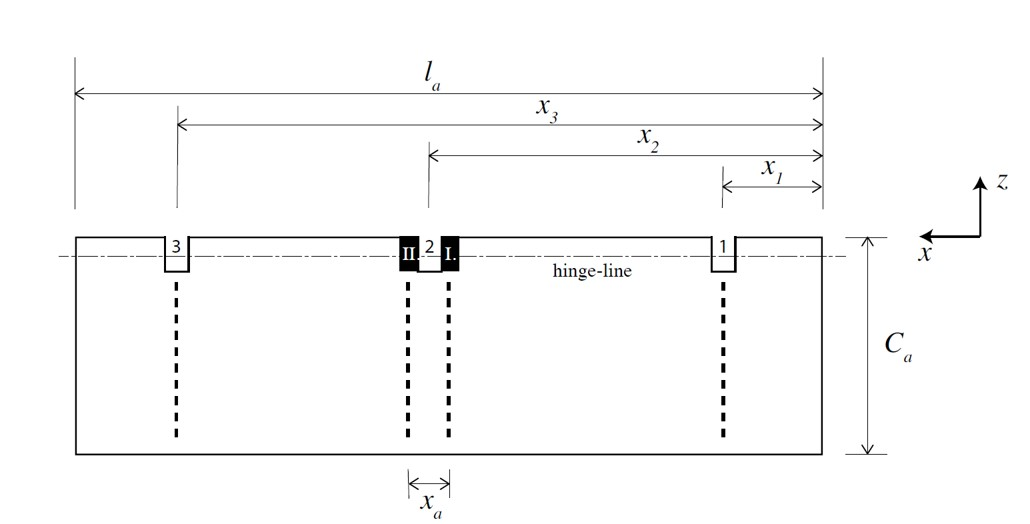
\includegraphics[width=8cm]{Images/Dimension_top_view.jpg}
\caption{Geometry and dimensions: Top view \cite{Assignment_description}.}
\label{fig:Dimensions_top_view}
\end{minipage}
\hspace{0.5cm}
\begin{minipage}[b]{0.45\linewidth}
\centering
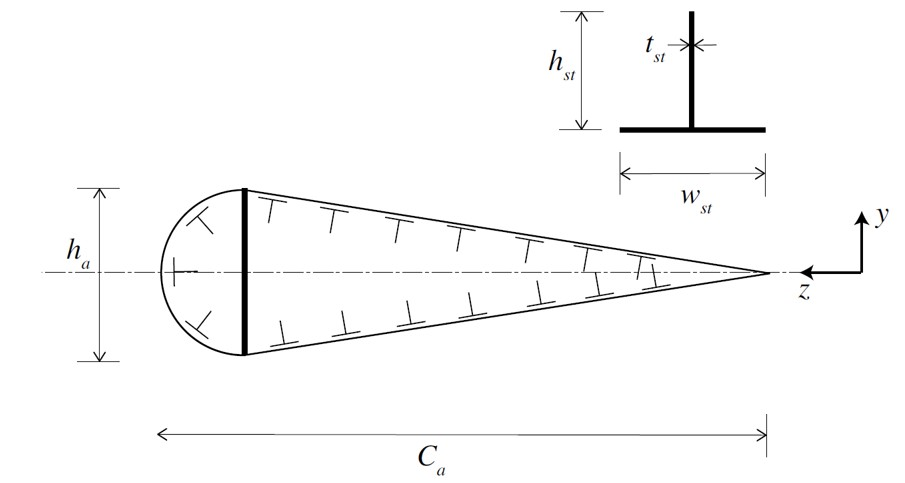
\includegraphics[scale=0.1]{Images/Dimension_side_view.jpg}
\caption{Geometry and dimensions: Side view \cite{Assignment_description}. }
\label{fig:Dimensions_side_view}
\end{minipage}
\begin{minipage}[b]{\linewidth}
\centering
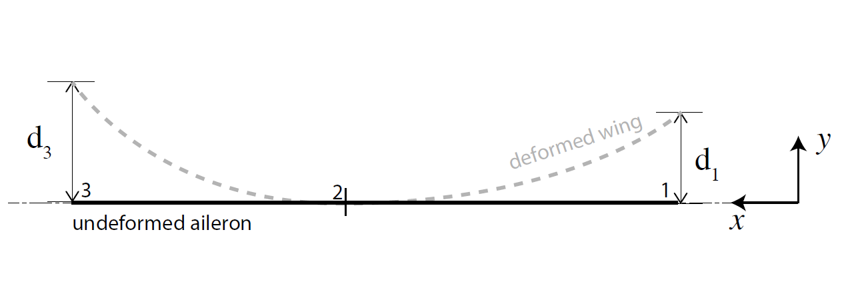
\includegraphics[width=7.5cm]{Images/Dimension_back_view.jpg}
\caption{Geometry of the deformed and undeformed aileron : Back view \cite{Assignment_description}.}
\label{fig:Dimensions_back_view}
\end{minipage}
\end{figure}

\begin{table}[]
\caption{Parameters of aileron of the Fokker 100 \cite{aircraft_data}}
\label{ParametersaileronF100}
\begin{tabular}{|l|l|l|l|}
\hline
\textbf{Property}                                                                       & \textbf{Symbol} & \textbf{Value} & \textbf{Unit} \\ \hline
Chord length aileron                                                           & C\_a   & 0.505 & m    \\ \hline
Span of the aileron                                                            & l\_a   & 1.611 & m    \\ \hline
x-location of hinge 1                                                          & x\_1   & 0.125 & m    \\ \hline
x-location of hinge 2                                                          & x\_2   & 0.498 & m    \\ \hline
x-location of hinge 3                                                          & x\_3   & 1.494 & m    \\ \hline
Distance between actuator 1 and 2                                              & x\_a   & 24.5  & cm   \\ \hline
Aileron height                                                                 & h      & 16.1  & cm   \\ \hline
Skin thickness                                                                 & t\_sk  & 1.1   & mm   \\ \hline
Spar thickness                                                                 & t\_sp  & 2.4   & mm   \\ \hline
Thickness of stiffener                                                         & t\_st  & 1.2   & mm   \\ \hline
Height of stiffener                                                            & h\_st  & 1.3   & cm   \\ \hline
Width of stiffener                                                             & w\_st  & 1.7   & cm   \\ \hline
Number of stiffeners (equally spaced along the periphery of the cross-section) & n\_st  & 11    & -    \\ \hline
Vertical displacement hinge 1                                                  & d\_1   & 0.389 & cm   \\ \hline
Vertical displacement hinge 3                                                  & d\_3   & 1.245 & cm   \\ \hline
Maximum upward deflection                                                      & \theta      & 30    & deg  \\ \hline
Load in actuator 2                                                             & P      & 49.2  & kN   \\ \hline
\end{tabular}
\end{table}






\subsection{Load case and free body diagrams}
The locations of the three hinges and the two actuators can be seen in \figautoref{fig:Dimensions_top_view}.
The aileron is attached to the wing via three hinges, numerically ordered from right to left in \figautoref{fig:Dimensions_top_view}. The second (middle) hinge is fixed in x-,y- and z-direction.
The first (right) and second (left) hinge are fixed only in y-direction.
The actuator that is numbered I in \figautoref{fig:Dimensions_top_view} is fixed.
At each hinge there are three reaction forces in x-,y- and z-direction. \\

\noindent A point load P acts at actuator II in negative y- and z-direction. Its direction is equal to a negative rotation around the x-axis that is equal to the maximum upward deflection angle. 
A distributed load q is present due to aerodynamic forces. Its direction is in negative y-direction, perpendicular to the symmetry plane of the aileron (x-,z-plane). The magnitude of the distributed load varies over the aileron surface in both x- and z-direction. 

\noindent These loads acting on the aileron in the relevant loading case can now be visualised. This is done in the free body diagrams for the top view, side view and back view. These can be seen in \figautoref{fig:FBD_top_view}, \figautoref{fig:FBD_side_view} and \figautoref{fig:FBD_back_view}.
\par
\begin{figure}[H]
\begin{minipage}[b]{0.45\linewidth}
\centering
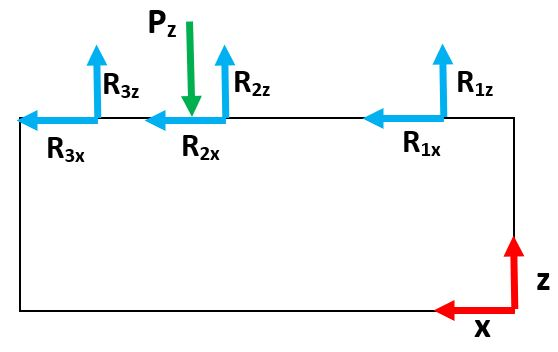
\includegraphics[width=6cm]{Images/New_FBD_top.JPG}
\caption{Free body diagram: Top view}
\label{fig:FBD_top_view}
\end{minipage}
\hspace{0.5cm}
\begin{minipage}[b]{0.45\linewidth}
\centering
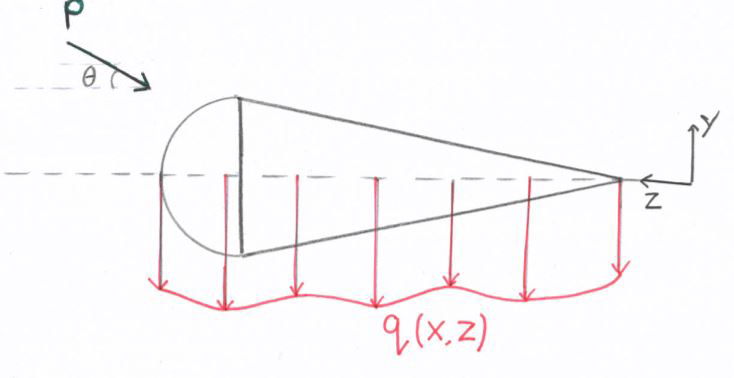
\includegraphics[width=0.95\textwidth]{Images/FBD_side_view.jpg}
\caption{Free body diagram: Side view}
\label{fig:FBD_side_view}
\end{minipage}
\begin{minipage}[b]{\linewidth}
\centering
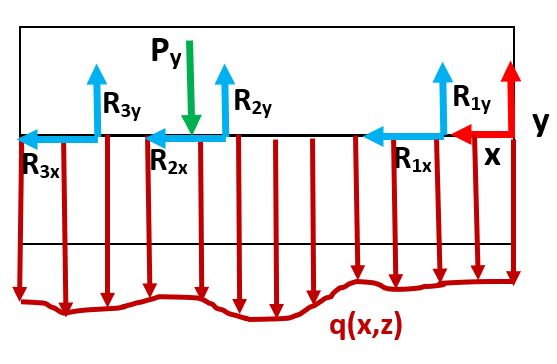
\includegraphics[width=5cm]{Images/New_FBD_back_view.JPG}
\caption{Free body diagram: Back view}
\label{fig:FBD_back_view}
\end{minipage}
\end{figure}

\newpage
\section{Numerical Model}
\label{sec:numerical_model}
\textit{This chapter will discuss the assumptions made in the development of the numerical model as well as the approach taken to calculate the internal stresses of the aileron.\\
Firstly the assumptions and idealisations are listed along with their arguments and significance. Secondly, the method that is used to make the simulation is explained. Furthermore, the load case and the governing equations of the numerical model are explained.}

\subsection{Assumptions and idealisations}
\label{subsec:assumptions_numerical}
The structure is idealised as a boom skin multi-cell beam structure. This assumption is reasonable, as the thickness of the skin is magnitudes smaller than the size of the structure, as well as the Moment of Inertia of a stringer is magnitudes smaller than its contribution to the bending stiffness by the parallel axis theorem. With this idealisation it is assumed that only the stiffeners carry normal stresses, while the skin only carries shear. Furthermore it is assumed that the material is behaving linearly in all load cases, this is a reasonable assumption if the maximum stress in the aileron stays below the yield stress of the material used.\\

\noindent As the structure is assumed to be thin walled with stringers in the direction of the x axis, compressive and tensile forces are only taken into account for this direction, as there are however no external forces acting in the x axis, the structure is assumed to be only in shear, bending, and torsion. These 3 can occur around all axes. However, bending around the y axis is neglected, as all 3 hinges are fixed in this direction and the moment of inertia for this bending is bigger than for the other directions while the forces causing it are smaller. Bending around the x axis is also neglected as the chord of the aileron is much shorter than the width of the aileron. Torsion is only considered around the x axis of the aileron as this direction has the smallest cross-section of the 3 possible cutting planes. Furthermore, shear in the x direction is not calculated, as it can be seen by inspection that no external forces are acting in the x axis. In addition, the weight of the aileron is neglected in all calculations. It is also assumed that the deformation of the aileron has no effect on the deformation of the wing.

\subsection{Load case decomposition}
\label{subsec:load_decomposition}
In the concerning loading scenario, two loads are present along with the bending of the aileron. These together cause reaction forces which cause deflection, twist of the structure and stresses in the structure. Instead of analysing the effects of the bending and the two loads simultaneously, the effects of multiple load cases are analysed separately. Afterwards these are added up to get to the total load decomposition. Three load cases are used in the model.

\subsubsection{First load case}
\noindent Firstly there is the deformation of the aileron, due to the wing-flex of the main wing. This deformation is described as bending around the z-axis. Naturally this causes a bending moment around the z-axis. Furthermore this causes reaction forces to appear in hinge 1 and 3 in the y-direction.\\

\noindent The aileron deformation is numerically interpolated using a natural cubic spline with three knots consisting of hinge 1, 2 and 3. Consequently there are two spline segments.

\subsubsection{Second load case}
\noindent The second load case consists of the aerodynamic load acting on the aileron. This is a non uniformly distributed load, varying in x- and z- direction and acting in negative y-direction. It introduces a bending moment around the x- and z- axis. Furthermore it causes torsion around the x-axis, due to its uneven distribution of the load itself. Finally there is also a shear stress in the y-direction. \\

\noindent The input data consists of values of the aerodynamic load along the aileron in x- and z-direction. Firstly this data is interpolated with the use of tensor product interpolation. Finally Gauss quadrature is used for 2D integration.

\subsubsection{Third load case}
\noindent The third and final load case that is being considered is the load acting on actuator II. This load causes bending around the z-axis and torsion around the x-axis. Furthermore, shear stress is introduced in the z- and y-axis.

\noindent For all these load cases the reaction forces can be calculated by setting a force and moment equilibrium.

\subsubsection{Decomposition}
\noindent When all of the loads acting on the aileron are known, normal (bending) stress and shear stress are calculated for each load case if they apply. Finally, using the principle of superposition, normal stress and shear stress are calculated as a result of all load cases and unified into a single load case. From this load case the maximum angle of twist, maximum deflections of the aileron at the leading- and trailing edge and the maximum stresses can be found.


\subsubsection{Governing equations}
\label{subsubsec:gov_eq_numerical}

In order to determine the torsion in the aileron, a thin-walled multi cell beam structure is assumed, as stated in \autoref{subsec:assumptions_numerical}. Using this assumption, the following equations can be applied. The first equation deals with the torsion experienced by each cell in the structure. Ultimately these can be summed to come to the overall torsion in the structure. This equations holds $n$ unknown shear values for $n$ cells \cite{the_book}.
\begin{equation}
    T_x=\sum_{k=1}^{N}=2 A_{r} q
\end{equation}
The second equation deals with the rate of twist experienced by the entire structure, which thus is the same for every cell. For the same $n$ cells this results in the same $n$ unknown shear values for $n$ cells.
\begin{equation}
    \frac{d \theta}{d x}=\frac{1}{2 A_{r}} \oint \frac{q d s}{G t}
\end{equation}
Consequently, this system of equations is used to calculate the resulting shear flow in the entire aileron structure from the applied torques. Knowing these shear flow values, the rate of twist can be calculated.\par
\noindent In order to analyse the bending of the aileron, it is assumed to behave as an ideal engineering beam, which deflection can be described by \eqautoref{eq:Beamformula} \cite{the_book}.

\begin{equation}
    \frac{d^2}{d x^2}w(x) = \frac{M_x}{E I_{zz}}
    \label{eq:Beamformula}
\end{equation}

\noindent The normal stresses in the beam can be calculated by \eqautoref{eq:stress_bending_x} and \eqautoref{eq:stress_bending_z} \cite{the_book}.

\begin{equation}
    \sigma_x = \frac{M_z y}{I_{xx}}
    \label{eq:stress_bending_x}
\end{equation}

\begin{equation}
    \sigma_z = \frac{M_x y}{I_{zz}}
    \label{eq:stress_bending_z}
\end{equation}
Furthermore, the shear in the cross section of the structure can be described by \eqautoref{eq:bending_shear} in which V is the internal shear force,  t the thickness of the skin and Q the first moment of area from the neutral axis\cite{the_book}. Q can be simplified with the use of boom idealisation, which is explained in \autoref{subsubsec:MoI}. 

\begin{equation}
    \tau = \frac{V Q}{I t}
    \label{eq:bending_shear}
\end{equation}

\noindent Finally, the shear flow in the structure resulting from the shear is defined by the product of this shear and the thickness of the sheet it flows through. This can be seen in \eqautoref{eq:shearflow}

\begin{equation}
\label{eq:shearflow}
    q=\tau t
\end{equation}
\subsection{Method}
As described in the previous section our model is divided in different load cases which are combined after all the calculations. The model itself is set up in separate modules. 
These will be explained in the next paragraphs. Everything is also made visible with a flow chart to make it clearer to understand the working principle of the simulation.

\subsubsection{Centroid}
Firstly, the centroid along the z-axis is calculated as a result of the geometrical parameters of the aileron structure. The x- and y-centroid are equal to zero, as the structure is symmetric around these axes.

\subsubsection{Structural idealisation}
\label{subsubsec:boom}
%Maybe include a sketch of the idealisation if we have the time
Structural idealisation is realised by applying boom idealisation. This is an assumption that simplifies the structure in such a way that the stiffeners are considered concentrations of area, called booms. They are the sole carriers of normal stresses. The stress acting over these booms is constant. Additionally, the skin carries the entire shear flow, which is constant in between a pair of booms.\\

\noindent The concerning aileron consists of eleven stiffeners, equally spaced along the periphery of the cross-section (y,z-plane). The stiffeners in the left part of the structure are equally spaced from each other with radial distance $d$. Furthermore, the stiffeners in the right part are equally spaced with distance $a$. A visualisation of the boom idealisation is shown in \autoref{fig:boom}.
This idealisation is used to calculate the moment of Inertia and also when calculating the shear flow due to shear loads.

\begin{figure}[H]
    \centering
    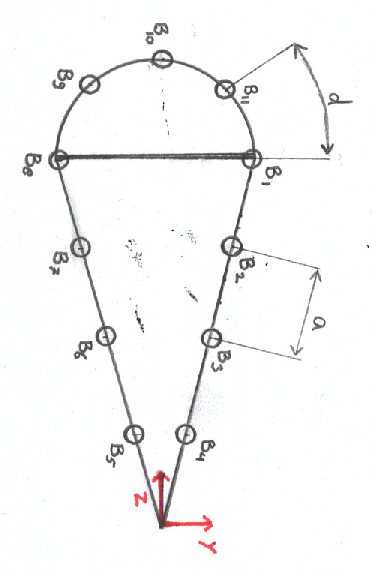
\includegraphics[width=6cm,angle=90]{Images/boom.pdf}
    \caption{Structural boom idealisation of the aileron structure}
    \label{fig:boom}
\end{figure}

\subsubsection{Moment of inertia}
\label{subsubsec:MoI}
The first and second moment of Inertia's around the x- and z-axes are calculated. This is done by taking the Steiner term for each boom \cite{the_book}. The formulas used for this are the following \eqautoref{MoI_xx}, \eqautoref{MoI_yy} and \eqautoref{MoI_zz}:
\begin{equation}
\label{MoI_xx}
    I_{x x}=\sum_{i=1}^{n} y_{i}^{2} B_{x_{i}}
\end{equation}

\begin{equation}
\label{MoI_zz}
    I_{z z}=\sum_{i=1}^{n} y_{i}^{2} B_{z_{i}}
\end{equation}

\subsubsection{Load cases}

There are three load cases considered for the concerning load scenario. These include all the loads acting on the aileron.
Firstly there is the aileron deformation due to the wing-flex of the main wing. Secondly, the aerodynamic load is considered, which is distributed over the aileron surface. Finally there is the discrete load $P$ acting on actuator $II$. All of these loads introduce reaction forces in hinges 1, 2 and 3. A more elaborate description and analysis is given in \autoref{subsec:load_decomposition}.

\subsubsection{Shear}
Shear flow experienced by the structure is caused by shear loads and torques. In this numerical model the shear flow distribution in the skin is calculated separately for external shear forces and external torques. This is done for each load case. Consequently the total shear flow distribution is determined by adding up the shear flow values. Knowing these values, the rate of twist around the x-axis can be calculated. This rate of twist is then numerically integrated over the span of the aileron to come to the total twist of the structure. For this, Gauss quadrature integration is used.
As is mentioned in \autoref{subsubsec:boom}, shear flows only through the skin.

\subsubsection{Normal stress}
Normal stresses are solely caused by the bending moment. As stated in \autoref{subsec:assumptions_numerical}, the numerical model only takes into account bending moment around the z-axis. The bending around x- and y-axis are neglected.
The normal stresses in each boom are determined from the bending moments caused by all three load cases. Then these are added up and this results in the total normal stress distribution in the structure.

\subsection{Flow chart}
The method of the simulation is also made visible with a flow chart (\autoref{flowchart}), in which the same chronological order (of the method) can be found. By following the numbers in the beginning of every square, it is clear that from the geometric properties first some necessary values are calculated (centroid, idealisation, moment of inertia). Afterwards the three load cases are analysed separately. Starting with the stresses induced by the wing deformation. Because this loading was not given it needs to be obtained in the opposite direction. From displacement to moment to stresses. To do this a linear system of equations and some boundary conditions are used.\\

\noindent For the two other load cases some extra inputs are needed, namely the loading itself. Despite the fact that these loads are solved in two different cases, their way of solving is the same. Namely analysing the load, solve for the reaction forces and the different internal loads and extracting the stresses from these internal loads.\\

\noindent All these elements are then combined together to get the ultimate load case from which the maximum stresses, angle of twist and deformations can be obtained.


\label{subsec:Flow_chart}
\begin{figure}[H]
    \centering
    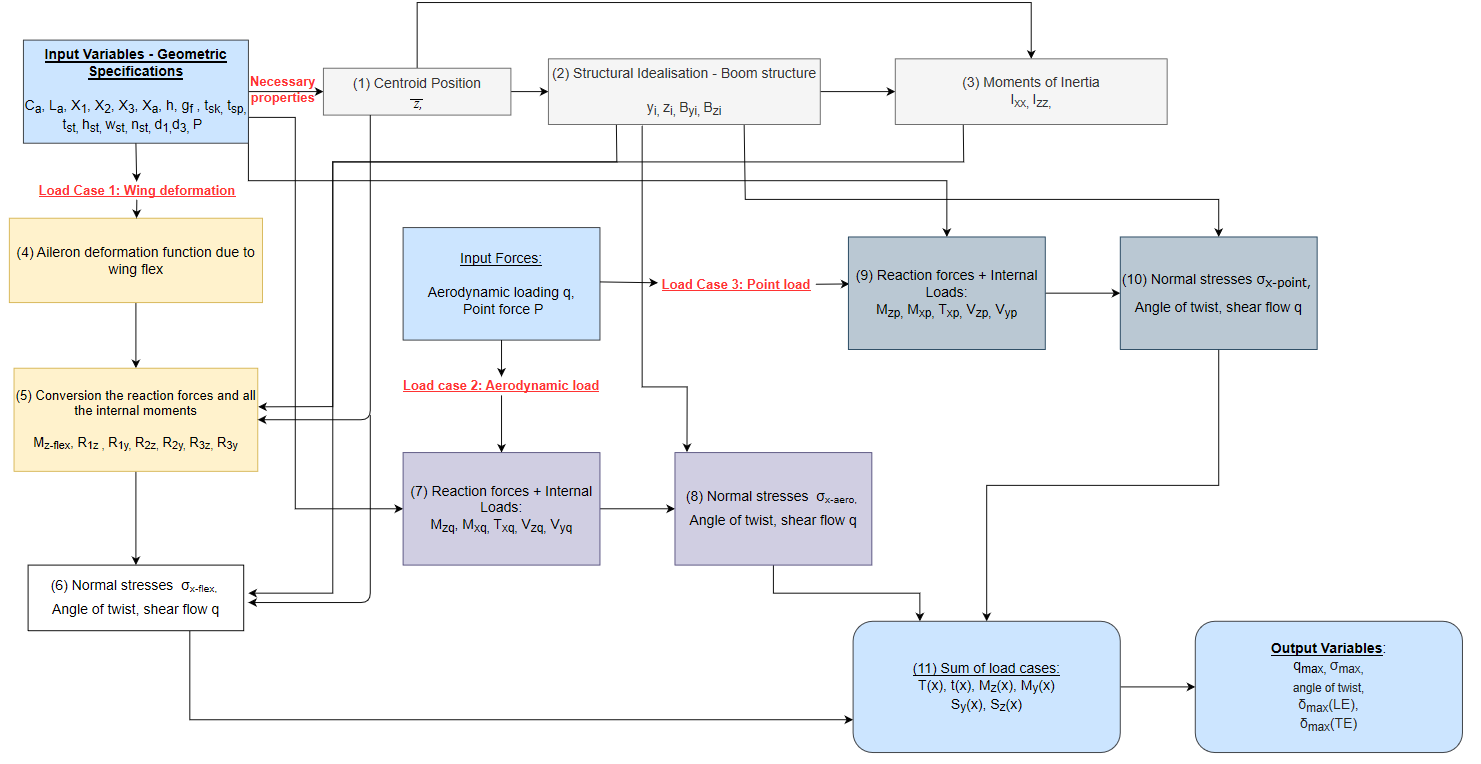
\includegraphics[width=23cm, angle=90]{Images/Flowchart3.PNG}
    \caption{Flowchart as illustration of the working principle of the simulation }
    \label{flowchart}
\end{figure}




















\newpage
\section{Verification Model}
\label{sec:verification_model}

\textit{This chapter will describe and analyse the given verification model. It will begin by presenting the motivation behind why the verification model is considered suitable to verify the numerical model. The following sections will discuss the assumptions and method used in the verification model. }

\subsection{Motivation}
The numerical model that will be developed by the team in the following weeks shall consist of implementing a different method than the one utilised in the given verification model to compute the required outputs. Due to the fact that different methods are used, if the results provided by the numerical model are consistent with the results provided by the verification model, it will be safe to assume that the numerical model is working correctly. This is why using this given verification model is beneficial in the verification process of the numerical model.

\subsection{Assumptions}
In the verification model, multiple assumptions are made. To prevent the need to repeat, all the assumptions used throughout the verification model are stated below with their explanations.\\
\begin{itemize}
    \item The aileron consists of only thin walled components.\\\\
    This is a valid assumption because the thickness of the skin and stiffeners are one order of magnitude smaller than the total structure. This assumption makes it easier to calculate the sheer flow in a cross section because it is not dependent on the thickness. Even though the thickness is not constant and shear flow peaks could occur, the assumption is still applicable because the contribution would be too small.\\
    \item The stringers are assumed to be point areas located on the skin.\\ \\
    This assumption makes the computation of the centroid easier and is applicable because the centroids of these stringers are not contributing largely to the the centroid of the whole structure. It also ensures the stringers do not have a moment of inertia around their own axis because this moment of inertia is neglectable with regards to the Steiner terms.\\
    \item The verification model also assumes an uneven number of stringers of which one is placed at the leading edge.\\\\
    This assumption ensures the the aileron is symmetric and the centroid is on the line of symmetry. When the necessity to cut the structure arises, the area of the stringer of the leading edge can be split in half.\\
    \item To compute torsional stiffness, skins and spar are assumed to carry bending stresses.\\ \\ This ensures that the shear flow varies between the booms and the booms of the idealisation have the area of the the stringers. This assumption splits up the the stringers and the skins and spar to be able to calculate shear flow. It is applicable because the resistance against shear of the stringers is neglectable. \\
    \item The spacing of the stringers is assumed to be constant along the skin of the aileron
    
\end{itemize}
\subsection{Bending stiffness calculations}
In order to be able to calculate bending stresses and stiffness, the respective properties need to be computed. These properties are the centroid and second moment of area of the aileron. \\ \\
To compute the centroid, using previously mentioned assumptions, it is necessary to know the stringer spacing. This can be done by dividing the length of the skin by the number of stringer. Then, by knowing the locations, the centroid can be calculated using \eqautoref{centroid}.
\begin{equation}
\label{centroid}
    \bar{x}=\frac{\int \tilde{x} d A}{\int d A} ;  \bar{y}=\frac{\int \tilde{y} d A}{\int_{A} d A}
\end{equation}

\noindent When the centroid is obtained, the second moment of area can be computed using the Steiner terms of the stringers, skins and spar, and the moments of inertia of the skins and spar. Combining these using formulae from literature, the total moment of inertia of the structure can be found.

\subsection{Torsional stiffness calculations}\label{subsec:torsstiffcalc}

For torsional stiffness, first the shear must be calculated. By drawing a sketch and making cuts, \eqautoref{qb} can be used:
\begin{equation}
\label{qb}
    q_{b}(s)=-\frac{1}{I_{z z}}\left(\int_{0}^{s} t y d s+\sum_{i=1}^{i \ni s_{s} \leq s} B_{i} y_{i}\right)+q_{b_{0}}
\end{equation}
\noindent Then the redundant shear flow can be calculated using the deflection formula, \eqautoref{dtheta}. 
\begin{equation}
\label{dtheta}
    \frac{d \theta}{d z}=\frac{1}{2 A_{i}} \oint \frac{q d s}{G t}=0
\end{equation}
Now that the shear through the structure is known, the torsional stiffness can be calculated using \eqautoref{T} and \eqautoref{Gdtheta} to combine both cells and a final torsional constant is found. 
\begin{equation}
\label{T}
    T=2 A_{1} q_{0,1} 1+2 A_{2} q_{0,2}
\end{equation}

\begin{equation}
\label{Gdtheta}
    G \frac{d \theta}{d z}=\frac{1}{2 A_{i}} \oint \frac{q d s}{t}
\end{equation}
\subsection{Deflection calculations}
\label{subsec:deflection_calculations}
In the provided verification model \cite{Verification_model_description}, the deflections of the flexural axis of the aileron are evaluated using the principle of stationary potential energy applied to a closed-section beam subject to lateral deflections and torsion. This was made possible by using the Rayleigh-Ritz method, which will be discussed next.

\noindent The motivation behind using the Rayleigh-Ritz method is that this is a well established method, frequently referenced in literature with applications in structural analysis. Furthermore, it is considered to be the basis/predecessor of the Finite Element Analysis and is assumed to be a good fit for analysing fairly uniform structures, such as an aileron. The method finds deflection functions that minimise the total potential energy $\Pi$, as defined by the principle of stationary total potential energy in \eqautoref{eq:total_potential_energy},

\begin{equation}
\label{eq:total_potential_energy}
    \Pi= U + V
\end{equation}

\noindent where $U$ is the total strain energy and $V$ is the work potential.\\

\noindent The Rayleigh-Ritz method delivers an optimal approximation of the solution, as opposed to the exact solution. Thus, the solution provided by this method is assumed to consist of a finite sum of basis functions, whose coefficients are selected in order to minimise a quantity, as explained in \cite{Verification_model_description}. \\

\noindent The first step taken in the process of using the Rayleigh-Ritz method to solve the problem at hand, was to apply the method to a simple, one-dimensional beam, that was subjected to only one lateral deflection assumed to be in the vertical direction. No twist was taken into account, and the boundary conditions were assumed to be homogeneous. A coordinate system centered at the leading edge of the root chord, with $x$ pointing outboard and $z$ acting as a symmetry axis, pointing towards the trailing edge, has been chosen. Then total strain energy $U$ and the work potential $V$ have been expressed for the previously described case and thus, an equation for the total potential energy $\Pi$ was derived. \\

\noindent Next, due to the fact that the principle of stationary total potential energy states that the total potential energy of a system is minimum when the system is in equilibrium, it results that the derivative of $\Pi$ with regards to any quantity should be zero. This is why it may be assumed at this stage of the process that the solution for the deflection $v$ may be expressed as a linear combination of a finite set of basis functions, as expressed in \eqautoref{eq:basis_functions},

\begin{equation}
\label{eq:basis_functions}
    v(\xi)=\sum_{i=0}^{N-1} a_{i} \mathbf{\Psi}_{i}(\xi)=\mathbf{a}^{T} \mathbf{\Psi}(\xi)
\end{equation}

\noindent where $N$ is the dimension of the function space of the set of basis functions, \textbf{a} denotes a vector that contains the $N$ coefficients and $\mathbf{\Psi}$ is the vector that contains the $N$ basis functions. Thus, the deflection is $v=\mathbf{a}^{T} \boldsymbol{\Psi}=\boldsymbol{\Psi}^{T} \mathbf{a}$. After substituting this into the previously derived equation for the total potential energy $\Pi$, the derivative $\frac{\partial \Pi}{\partial \mathbf{a}}$ was expressed and set equal to 0, for the reason mentioned above. The worked out form of this equation is 

\begin{equation}
\label{eq:derivative}
    \frac{8 E I}{l_{a}^{3}} K_{1} \mathbf{a}=\frac{l_{a}}{2} K_{2}
\end{equation}

\noindent where $K1$ and $K2$ are matrices, expressed as

\begin{equation}
\label{eq:K1}
    K_{1}=\int_{-1}^{1} \frac{d^{2} \mathbf{\Psi}}{d \xi^{2}} \frac{d^{2} \mathbf{\Psi}^{T}}{d \xi^{2}} d \xi
\end{equation}

\begin{equation}
\label{eq:K2}
   K_{2}=\int_{-1}^{1} q_{a} \mathbf{\Psi} d \xi
\end{equation}

\noindent The next step consisted of choosing basis functions in such a way that their linear combination would satisfy the homogeneous boundary conditions imposed. A case with $N_{bc}$ boundary conditions of the form $\mathcal{L}\left\{v\left(\xi_{i}\right)\right\}=0, \quad 0 \leq i<N_{b c}$ was considered. Furthermore, two types of boundary conditions have been taken into account: a simple support $\rightarrow v\left(x_{1}\right)=0$ and a first order condition $\rightarrow v^{\prime}\left(x_{2}\right)=0$. In order to account for the $N-N_{bc}$ free variables, the form of the boundary conditions has been modified to

\begin{equation}
\label{eq:new_form_of_BC}
    \Upsilon_{1} \mathbf{\bar{a}}+\Upsilon_{2} \mathbf{\hat{a}}=0
\end{equation}

\noindent where $\mathbf{\bar{a}}=-\Upsilon_{1}^{-1} {\Upsilon}_{2} \hat{\mathbf{a}}=\Upsilon \hat{\mathbf{a}}$ denotes the first $N_{bc}$ coefficients and $\mathbf{\hat{a}}$ denotes the other $N-N_{bc}$ coefficients. Furthermore, $\Upsilon_{1}$ is a $N_{b c} \times N_{b c}$ matrix and $\Upsilon_{2}$ a $N_{b c} \times\left(N-N_{b c}\right)$ matrix, with entries expressed by

$$
\begin{aligned}
\Upsilon_{1_{1 j}} &=\mathcal{L}\left\{\psi_{j}\left(\xi_{i}\right)\right\} \\
\Upsilon_{2_{i j}} &=\mathcal{L}\left\{\psi_{j+N_{b c}}\left(\xi_{i}\right)\right\}
\end{aligned}
$$

\noindent Using this knowledge, differentiating the equation for the total potential energy $\Pi$ with respect to $\mathbf{\hat{a}}$ and setting it equal to 0 results in an $N_{b c} \times N_{b c}$ system of equations:

\begin{equation}
\label{eq:first_system}
    \frac{8 E I}{l_{a}^{3}}\left(\Upsilon^{T} K_{1}^{(1,1)} \Upsilon+\Upsilon^{T} K_{1}^{(1,2)}+K_{1}^{(2,1)} \Upsilon+K_{1}^{(2,2)}\right) \hat{\mathbf{a}}=\frac{l_{a}}{2}\left[K_{2}^{(1)} \Upsilon+K_{2}^{(2)}\right]
\end{equation}

\noindent The next step in the process of applying the Rayleigh-Ritz method, was to account for the more general case, by introducing non-homogeneous boundary conditions of the form $\mathcal{L}\left\{v\left(\xi_{i}\right)\right\}=f\left(\xi_{i}\right)$. Thus, \eqautoref{eq:new_form_of_BC} becomes $\Upsilon_{1} \mathbf{\bar{a}}+\Upsilon_{2} \mathbf{\hat{a}}=\mathbf{f}$, where the vector $\mathbf{f}$ includes the boundary conditions. Furthermore, the system of equations found in \eqautoref{eq:first_system} has a new form that accounts for the non-homogeneous boundary conditions, through the term $F$:
\begin{equation}
    \label{eq:second_system}
    \frac{d \Pi}{d \hat{\mathbf{a}}}=\frac{8 E I}{l_{a}^{3}}\left(\Upsilon^{T} K_{1}^{(1,1)} {\Upsilon}+\Upsilon^{T} K_{1}^{(1,2)}+K_{1}^{(2,1)} {\Upsilon}+K_{1}^{(2,2)}\right) \hat{\mathbf{a}}=-\frac{8 E I}{l_{a}^{3}}\left({\Upsilon}^{T} K_{1}^{(1,1)} F+K_{1}^{(2,1)} F\right)+\frac{l_{a}}{2}\left[K_{2}^{(1)} {\Upsilon}+K_{2}^{(2)}\right]
\end{equation}

\noindent At this stage of the process, a set of monomials was selected as the set of basis functions.
The following step consisted of the introduction of the torque distribution in the solution. This means that at this moment in the process, on top of the lateral deflections introduced, a torsional deflection is taken into account. The main steps, as described before are followed. The solutions are assumed to be given by:

\begin{equation}
    \begin{aligned}
v(\xi) &=\sum_{i=0}^{N-1} a_{i} \psi_{i}(\xi)=\mathbf{a}^{T} \mathbf{\Psi}(\xi) \\
\phi(\xi) &=\sum_{i=0}^{N-1} c_{i} \psi_{i}(\xi)=\mathbf{c}^{T} \mathbf{\Psi}(\xi)
\end{aligned}
\end{equation}


\noindent Three types of boundary conditions have been used, namely a simple support $v(x_1,z_1) = f_1$, a first-order support on the slope of the flexural axis $v^{\prime}(x_2)=f_2$ and a twist constraint $\phi(x_3)=f_3$. Similarly to the procedure used before to obtain \eqautoref{eq:new_form_of_BC}, the following equation is obtained:

\begin{equation}
\label{eq:new_form_of_BC_torsion}
    \Upsilon_{1} \mathbf{\bar{a}}+\Upsilon_{2} \mathbf{\hat{a}}+\Upsilon_{3} \mathbf{\bar{c}}+\Upsilon_{4} \mathbf{\hat{c}}=0
\end{equation}

\noindent where $\Upsilon_{1}$ is a $N_{bc}$ x $N_a$ matrix, $\Upsilon_{2}$ a $N_{bc}$ x $(N - N_a)$ matrix, $\Upsilon_{3}$ a $N_{bc}$ x $N_c$ matrix and $\Upsilon_{4}$ a $N_{bc}$ x $(N - N_c)$ matrix, $N_a + N_c=N_{bc}$. Futhermore, $\mathbf{\bar{c}} \text{ and } \mathbf{\hat{c}}$ have been defined as the vectors that contain the first $N_c$ coefficients, respectively the remaining $N-N_c$ coefficients $c_i$. 

\noindent The last and most important step of applying the method to the problem at hand consists of including the second shear lateral deflection, in the $z$ direction. At this point, the expression for the total potential energy is:

\begin{equation}
    \label{eq:total_potential_energy_final}
    \begin{aligned}
\Pi=U+V=& \frac{4 E I_{z z}}{l_{a}^{3}} \int_{-1}^{1}\left(\frac{d^{2} v}{d \xi^{2}}\right)^{2} d \xi+\frac{4 E I_{y y}}{l_{a}^{3}} \int_{-1}^{1}\left(\frac{d^{2} w}{d \xi^{2}}\right)^{2} d \xi+\frac{G J}{l_{a}} \int_{-1}^{1}\left(\frac{d \phi}{d \xi}\right)^{2} d \xi \\
&-\int_{0}^{l_{a}} q_{a} v d x-\int_{0}^{l_{a}} q_{b} w d x-\int_{0}^{l_{a}} \tau_{x} \phi d x
\end{aligned}
\end{equation}

\noindent where $v$ accounts for the deflection in $y$-direction, $w$ accounts for the deflection in $z$-direction and $\phi$ accounts for torsion. Furthermore, $q_a$ represents the distributed load in $y$-direction, $q_b$ represents the distributed load in $z$-direction and $\tau_x$ represents the total distributed torque. At this point, it was assumed that the solutions are expressed as:

\begin{equation}
    \begin{array}{l}
{v(\xi)=\sum_{i=0}^{N-1} a_{i} \psi_{i}(\xi)=\mathbf{a}^{T} \mathbf{\Psi}(\xi)} \\
{w(\xi)=\sum_{i=0}^{N-1} b_{i} \psi_{i}(\xi)=\mathbf{b}^{T} \mathbf{\Psi}(\xi)} \\
{\phi(\xi)=\sum_{i=0}^{N-1} c_{i} \psi_{i}(\xi)=\mathbf{c}^{T} \mathbf{\Psi}(\xi)}
\end{array}
\end{equation}

\noindent It was assumed that the same set of basis functions, consisting of monomials, as well as the same number $N$ of coefficients are used for the three types of deflections.

\noindent Similarly to the previous steps, $N_{bc}$ boundary conditions were defined next. This time, seven types of boundary conditions have been considered:
\begin{itemize}
    \item a simple support in the $y$-direction $\rightarrow v\left(x_{1}, y_{1}, z_{1}\right)=f_{1}$
    \item a simple support in the $z$-direction $\rightarrow w\left(x_{2}, y_{2}, z_{2}\right)=f_{2}$
    \item a simple support in an arbitrary direction, oriented within the $yz$-plane described by $\theta_i$ $\rightarrow \cos \left(\theta_{3}\right) v\left(x_{3}, y_{3}, z_{3}\right)+\sin \left(\theta_{3}\right) w\left(x_{3}, y_{3}, z_{3}\right)=f_{3}$
    \item a first-order support on the slope of the flexural axis around the $z$-axis $\rightarrow v^{\prime}\left(x_{4}\right)=f_{4}$
    \item a first-order support on the slope of the flexural axis around the $y$-axis $\rightarrow -w^{\prime}\left(x_{5}\right)=f_{5}$
    \item a first-order support in an arbitrary direction, oriented within the $yz$-plane described by $\theta_i$ $\rightarrow -\cos \left(\theta_{6}\right) w^{\prime}\left(x_{6}\right)+\sin \left(\theta_{6}\right) v^{\prime}\left(x_{6}\right)=f_{6}$
    \item a twist constraint $\rightarrow \phi\left(x_{7}\right)=f_{7}$
    
\end{itemize}

\noindent Due to the fact that $N$ basis functions were used, the number of free variables was equal to $3N- N_{bc}$, as there were three types of deflections and thus 3 functions that needed to be approximated. The model initially uses 20 basis functions \cite{Verification_model_description}. After establishing the boundary conditions, the discretisation process could begin. Thus, similarly to the way \eqautoref{eq:new_form_of_BC} and \eqautoref{eq:new_form_of_BC_torsion} have been derived, the following was obtained:

\begin{equation}
    \label{eq:new_form_of_BC_final}
    \Upsilon_{1} \mathbf{\bar{a}}+\Upsilon_{2} \mathbf{\hat{a}}+\Upsilon_{3} \mathbf{\bar{b}}+\Upsilon_{4} \mathbf{\hat{b}}+\Upsilon_{5} \mathbf{\bar{c}}+\Upsilon_{6} \mathbf{\hat{c}}=0
\end{equation}

\noindent Following the procedure explained in the first step (\eqautoref{eq:total_potential_energy} to \eqautoref{eq:first_system}), a final discretised model/governing equation could be derived from \eqautoref{eq:new_form_of_BC_final}. This discretised model is being fed into the program in order for the computer to be able to provide a solution.  

\subsection{Stress calculations}
As explained in \autoref{subsec:torsstiffcalc}, the shear flow distributions $q_b(s)$ at any point can be calculated. These can be converted to shear stresses $\tau$ by dividing by the local thickness. 
Furthermore, the direct stress due to the moment $M_y$ and $M_z$ can be calculated on any location using \eqautoref{eq:sigma_xxz} and \eqautoref{eq:sigma_xxy}, which were found in the verification model \cite{Verification_model_description}.

\begin{equation} \label{eq:sigma_xxz}
    \sigma_{xx}(z) = M_y \frac{z - \Bar{z}}{I_{yy}}
\end{equation}

\begin{equation} \label{eq:sigma_xxy}
    \sigma_{xx}(y) = M_z \frac{y}{I_{yy}}
\end{equation}

\noindent Then, the stresses can be combined into Von Mises stress distributions using \eqautoref{eq:vonmises}, also found in the verification model \cite{Verification_model_description}.

\begin{equation}\label{eq:vonmises}
\sigma_{vm} = \sqrt{\frac{(\sigma_{xx}-\sigma_{yy})^2+(\sigma_{yy}-\sigma_{zz})^2+(\sigma_{zz}-\sigma_{xx})^2}{2} + 3 (\tau_{xy}^2+\tau_{yz}^2+\tau_{xz}^2)}
\end{equation}

\subsection{Program description}
The program consists of 5 parts, which will each be discussed. \\

\noindent In part 1, the parameters are defined. These are the parameters that can be changed to perform verification with our model. \\

\noindent In part 2, the bending properties are established. This is done through defining a cross-section object, which is then used to calculate its bending properties. For this, several parameters can be reviewed, such as the location of the centroid, cross sectional area and stringer coordinates, and the moment of inertia about the y-axis and z-axis.\\

\noindent In part 3, the torsional properties are established for the cross-section object. These include the shear centre and torsional constant $J$, which can be reviewed. \\

\noindent In part 4, the $N$ number of basis functions will be set up, and some other material properties $E$ and $G$ are defined. Then, the aileron object is created using the energy method. Furthermore, boundary conditions and external loads will be defined, which have been described in section \ref{subsec:deflection_calculations}. Then the deflections are computed. These deflections in y and z are then plotted to check, and the values of shear force, torque and moments can be evaluated. Also, all the matrices and coefficients used in the energy method can be evaluated.\\

\noindent In part 5, the stress distributions are computed. These are separated in the shear flow, the direct stress and the Von Mises stress. These are plotted, and the values can be evaluated for each region, as previously specified.
\newpage
\section{Verification}
\label{sec:verification}
%In this chapter, we need to write about the types of unit testing (a little something for each of them) and maybe come up with some more
\textit{To ensure a working simulation, it is paramount to verify the model. This chapter will discuss how the team plans to perform the verification of the numerical model that will be implemented in the following weeks, through unit, integration and system testing.}

\subsection{Step by step model verification through unit testing}
A systematical approach to the verification is important to prevent issues as the program grows. To make sure nothing is overlooked, the model and its code will be verified in steps, through unit testing. In order to ensure a test coverage that approaches 100\% for the final program, the team aims to design and implement unit tests for each of the main functions, as presented in the flowchart in section \autoref{subsec:Flow_chart}. This will preferably be done right after a certain function has been implemented, in order to maximise efficiency and minimise the chance of finding out about a bug in the code late into the process and not being able to locate it. Automated unit tests will be implemented using Pytest, for the case where reasonable assertions can be expressed- when hand calculations can be performed. For the other case, manual unit testing will be performed and documented. An overview of the proposed unit tests will be presented next. 

\paragraph{Centroid}
\\The unit test to check for the correct centroid will be conducted as follows. The centroids of the separate components will be calculated by hand and by the numerical model. These will be compared. If they are correct, the model will be asked to compute the centroid of the whole structure. The easiest test to see whether this is correct is to verify that the centroid is on the line of symmetry. If it is, it needs to be compared to the centroid computed by hand to ensure the right centroid location. Also, tests for extreme situations will be performed to check for the right method.

\paragraph{Structural idealisation}\\
The module that computes the boom locations and areas can be checked in a similar fashion. By checking the centroid module and ensuring the correct input, again the result of the model can be compared with the outcome of calculations on paper. This then confirms the correct idealisation.

\paragraph{Moment of Inertia}\\
Similarly, to check the Moment of Inertia calculations, a simple boom discretisation with a known Moment of Inertia will be performed. This will then be confirmed using hand calculations. Then, the Moment of Inertia of the more difficult structure can be computed.

\paragraph{Reaction forces}\\ To check whether the program uses the correct forces and moments looking at the outputs will shed light on obvious mistakes. The aileron has to be in static equilibrium, meaning that the sum of forces in all directions and resultant moments in all directions must be zero. This is also applicable to all different sections. Therefore if this is not the case it is a clear show of mistakes in the program.

\paragraph{Interpolation tool}\\
The interpolation tool is used to approximate the value of a function, which is sampled at discrete grid points, when the point of interest does not coincide with a grid point. To check the module, a simple function can be used. The interpolation of for example a sine function can be easily compared to the output of the module. This can then later be used to compute accuracy.

\paragraph{Integration tool}\\
The Integration procedures for 1 and 2 dimensional cases are tested against analytically calculated integrals of simpler univariate or multivariate functions.



\subsection{Integration testing}
After each of the main functions have been tested using unit tests, it is time to verify to what extent do these units work together within the code, as some possible bugs may not be identified at the unit level itself.

\subsection{System Testing}
System testing represents the verification procedure of the program as a whole. This may be performed after the unit and integration testing. Due to the fact that the final program will be complex, system testing will be manually performed, as opposed to being automated. The system tests that are planned to be performed will be presented next.

\subsubsection{Using different input variables}
By using different input variables, that have different magnitudes, signs or meanings, the program can be checked for mistakes. This will be done by checking that the change produced in the output is consistent with the change expected from theory.   

\subsubsection{Using more mesh poin}
By using a larger amount of mesh 
At the last stage of the numerical model the aileron is discretised by being cut into segments along the span
of the aileron and the stresses at those points are then calculated. A test can be performed that makes these
segments smaller and smaller. The values of the stresses should eventually converge to the same values

\subsubsection{Maximum stress}

\subsubsection{Comparison with the given verification model}
The final system test that will be performed will consist of comparing the outputs of the designed numerical model with those delivered by the verification model. This will be done by changing the input variables in the verification model to those corresponding to the Fokker 100. Due to the fact that many different assumptions have been made both in the team's numerical model and in the given verification model, as different methods have been used, a perfect match of the output data of the two programs is not required. However, a very close result with minor to no differences should be observed with regards to the result of the verification model, in order to be able to state that the numerical model is indeed correct. 




\subsubsection{Verification of code} The verification of the code can be performed during and after the coding itself. By paying attention to syntax errors and general coding errors in the modules, they can be filtered out before the size of the program gets overwhelmingly big. The compiler will announce most of the errors and stop the program making it easy to observe coding errors. However, detecting errors like wrong indices, incomplete lists or inattentive mistakes are less easy to find. Therefore, keeping an eye on these whilst working on the models, will make the whole process a lot easier. A check for this is recalculating by hand, given the same input. If the output is the same, the module or program works the way it is supposed to. To ensure redundancy, multiple inputs will be used.
\subsubsection{Verification of calculations}
As modules, they will be checked for mistakes in calculations. These tests will show whether the modules function correctly so that they can be eliminated as source of the problem when combined with the other parts of the problem. Because these modules have a limited number of functionalities, they can easily be verified by a combination of pytest and computing the results by hand, or using unit tests. Working this way, python can compare the output of the module with result that was calculated by hand and directly stop the program if it is incorrect.\\ \\
The next step is testing for errors in the merger of modules. This is not as straight-forward as the checking of modules since there are numerous ways for the program to run through the modules. The main way of testing is by checking inputs and outputs along the way. If the output of a certain module fits with the input of the next, the link works the way it is supposed to. After this test, longer links of modules can be tested with given inputs and recalculations by hand.

\subsubsection{Accuracy of testing}
It is expected that the results of the unit tests won't match up exactly with the hand-calculated, because of rounding errors and the inexact representation of real numbers on a computer. Thus the unit tests will succeed if the difference between the results is less than 0.1\%. This limit is considered sufficiently small to ensure accurate enough calculations in later stages of the analysis. Furthermore, the interpolation and and integration procedures are tested for their order of accuracy. For this they will be run for different grid spacings, and the rate of decrease of error is observed. These tests will succeed if the order of accuracy matches the expected order of accuracy of the used method.

\subsection{Comparison}
After making sure the program works as required, the results can be compared to the results of the verification model, assuming the model does not contain faults. By again checking results during the program, discrepancies can be identified. Logically, if the first output is relatively close to the expected output from the verification model, and the second output is not, something is wrong in the numerical model. This way the verification model can be used as a very close approximation of what the numerical model should be. In order to ensure these tests will yield the actual order of accuracy of the used scheme, the functions $f$ used in testing are chosen such that $f \in C^{\infty}$. 

\newpage
\section{Validation}
\label{sec:Validation}
%maybe think about more tests/explaations of discrepancies
\textit{Once the numerical model is verified to work, it is crucial to also validate the model. This is done by comparing results to real life measurements, or in this case a Finite Element Model (FEM) of the aileron of the Boeing 737, which very closely resembles reality.}

\subsection{The Validation Model} 
The validation model that is given is a FEM. This model accounts for three load cases: the bending of the aileron without loads applied to it, the bending of the aileron with loads applied, and the unbent aileron with the loads applied. Out of the three, the second load case is of the highest importance, since the numerical model accounts for the case of bending with applied loads.

\subsection{Comparison of Numerical Model and Validation Model}
The results that can be retrieved from the validation model are the following: Von Mises stress, S12, nodal displacement and reaction forces, evaluated using a significantly high number of predefined points in the aileron, in the order of 10000 \cite{Assignment_description}, \cite{SVV_Validation_Data_2020}. These results therefore will be compared with the numerical model. For this, the numerical model's parameters will have to be adjusted. The physical configuration of the aileron has to be changed to that of the aileron implemented on Boeing 737, and the aerodynamic load has to be changed to the constant distributed load as specified in the reader.\\

From the data given in the validation model, the Von Mises stress values can be used in order to calculate the magnitude and position of the maximum stress in the aileron. Furthermore, from the nodal displacement may be used in the comparison and validation of the twist of the aileron, as well as the deflection of the hinge line, as computed using the numerical model. Thus, validation tests may be created for the three main outputs of the numerical model: 
\begin{itemize}
    \item \textbf{Maximum stress} $\rightarrow$ a direct comparison between the results provided by the numerical model and the values of the Von Mises stress provided by the validation model may be performed in this case. This is due to the fact that in the data given, the magnitude of the minimum as well as the maximum stress in the aileron is provided, together with the node number and position where these occur. Furthermore, a direct comparison of the S12 data from the FEM and shear stress distributions that may be produced by the numerical model can also be made. 
    
    \item \textbf{Deflection of the hinge line} $\rightarrow$ using the fact that the nodal positions are given in the data, and the geometry of the aileron is known, the points/nodes that lay on the hinge line of the aileron can be identified. The deflection caused by bending in the hinge line can be found by comparing the locations of the first and last node on the hinge line of the aileron, in span-wise direction. This deflection will then be compared with the one provided as an output by the numerical model.
    
    \item \textbf{Twist} $\rightarrow$ in order to extract information about the twist from the data given in the validation model, three cross-sections of the aileron, so data at three different positions in span-wise direction will be inspected, namely: at the root, at hinge 2 and at the tip of the aileron. The hinge line connects these three sections, and thus it represents a good choice for the rotation axis with respect to which the twist can be found. The position of the leading edge and trailing edge, as well as the rotation/orientation of the chord line of the three sections will be used to extract the values for the twist. These values may then be compared to the twist of the aileron provided by the numerical model.  
    
\end{itemize}


\subsection{Explanation of Discrepancies}
In the aerospace engineering field, it is common practice to take into account significantly high safety factors when designing structures. These factors are typically required to be around 50\% \cite{safety_factors}. Thus, it makes sense to impose an upper limit of the allowed differences between the results of the validation model and the results of the numerical model of 5\%, as this represents 10\% of the assumed safety factor. There are a couple sources of discrepancies between the given validation model and the proposed numerical model that make up for the main differences. The considered sources of discrepancies are:

\begin{itemize}
    \item The assumptions made in the numerical model that do not resemble reality, such as idealisations in moment of inertia calculations, by using the boom-theory, assumptions on the linearity of the material, and neglecting certain deflections.
    \item The inaccuracies due to discretisation in the numerical model.
    \item The assumptions made in the FEM that do not resemble reality. There are 2 major assumptions in this regard: The stringers are not placed in the FEM, but are 'smeared out' over the skin, and the aerodynamic load is applied at 11 discrete nodes, instead of a continuous load.
    \item The inaccuracies due to discretisation in the FEM. Finite Element Analysis (FEA) works with a lot of nodes, which reduces the inaccuracies due to the approximations made, but they still result in differences with regards to reality.
\end{itemize}

%Discrepancy: In the FEM, the aerodynamic load has been applied at 11 discrete nodes. This is different than in our system
%Significant discrepancy: In the FEM, the stringers are 'smeared out' over the skin, instead of our system of booms


%Requirements for this section:
%Proposed validation tests good, creativity shown, very well described. 
%Validation data is optimally used
%Plan for assessing/addressing discrepancies is consistent with description of assumptions and their effects, and the validation data
\newpage
%\input{Chapter5.tex}
%\newpage
%\input{Chapter6.tex}
%\newpage
%\section{Conclusion} 
\label{conclusion}





%\newpage
\appendix
\addcontentsline{toc}{section}{Appendices}
\section*{Appendices}
\section{Task allocation}
\begin{center}
    

\begin{table}[H]
\centering
\begin{tabular}{l|c|c|c|c|c|c|c|}

\cline{2-8}
\textbf{}                                  & \multicolumn{1}{l|}{\textbf{Student}} & \multicolumn{1}{l|}{Bram} & \multicolumn{1}{l|}{Menno} & \multicolumn{1}{l|}{Wieger} & \multicolumn{1}{l|}{Yara} & \multicolumn{1}{l|}{Florina} & \multicolumn{1}{l|}{Malte} \\ \hline
\multicolumn{1}{|c|}{\textbf{Task}}        & \textbf{Time (h)}                     &                           &                            &                             &                           &                              &                            \\ \hline
\multicolumn{1}{|l|}{Loading cases}        & 13                                     &   1                        &                            & 6                        &                           &                              & 6                          \\ \hline
\multicolumn{1}{|l|}{Numerical model}      & 20                                    & 9                         &                            & 6                           &                           &                              & 5                          \\ \hline
\multicolumn{1}{|l|}{Verification model}   & 17                                   &                            & 5                          &                             & 5                         & 7                            &                            \\ \hline
\multicolumn{1}{|l|}{Verification}         & 19                                     &     4                      &                            &  2                           & 6                         & 4                            &      3                      \\ \hline
\multicolumn{1}{|l|}{Validation}           & 9                                     &                           & 5                        &                             & 1                          & 3                            &                            \\ \hline
\multicolumn{1}{|l|}{General reporting}    & 13                                     &                 &                 4           &                             & 4                         & 4                            &        1                    \\ \hline
\multicolumn{1}{|c|}{\textbf{Total hours}} &         \textbf{91}                              & 14                        & 14                          & 14                          & 16                         & 18                           & 15                          \\ \hline
\end{tabular}
\caption{The task division and hours of working for the simulation plan.}
\end{table}
\end{center}
\vspace{-10mm}
\section{Gantt chart}
A Gantt chart has been constructed in order to help visualize the distribution of the workload for the entirety of the project. This will aid in keeping the team on track.
\begin{center}
\begin{ganttchart}[vgrid={draw=none,draw=none},%
            %today=15,%
            %today offset=.5,%
            %today label=Heute,%
            %progress=today,%
            y unit title=0.7cm,
            y unit chart=0.6cm,
            bar incomplete/.append style={fill=red},%
            progress label text=  {\quad\pgfmathprintnumber[precision=0,verbatim]{#1}\%}%
            ]{1}{20}
\gantttitlecalendar*[time slot format=isodate]{2020-02-10}{2020-02-28}{year, month} \\
\gantttitlelist{10,...,28}{1}\\
\ganttgroup{Total Duration}{1}{19} \\
 %%%%%%%%%%%%%%%%%Phase-1
\ganttgroup{Preparation}{1}{3} \\
\ganttbar{Reading}{1}{3} \\
\ganttlinkedbar{Introduction lecture}{2}{2}  \ganttnewline
%%%%%%%%%%%%%%%%%Phase-2
\ganttgroup{Simulation plan}{3}{5} \\
\ganttlinkedbar{Loading}{3}{4} \\
\ganttlinkedbar{Numerical model}{3}{4} \ganttnewline
\ganttlinkedbar{Verification model}{3}{4} \ganttnewline
\ganttlinkedbar{Verification}{3}{5} \ganttnewline
\ganttlinkedbar{Validation}{4}{5} \ganttnewline
\ganttlinkedbar{General reporting}{3}{5} \ganttnewline
 %%%%%%%%%%%%%%%%%Phase-3
\ganttgroup{Report}{6}{19} \\
\ganttbar{Evaluate and alter Simulation plan}{6}{8} \\
\ganttlinkedbar{Coding modules centroid, MoI, boom discretisation}{6}{9} \ganttnewline
\ganttlinkedbar{Coding modules load cases}{7}{10} \ganttnewline
\ganttlinkedbar{Verification}{8}{16} \ganttnewline
\ganttlinkedbar{Validation}{15}{19}\ganttnewline
\ganttlinkedbar{General reporting}{6}{19}\ganttnewline
%%%%%%%%%%%%%%%%%%%%%%%%%%%%%%%%%%%%%%%%%%%%%%%%%%%%%%%%%%%%%%%

\end{ganttchart}

    
\end{center}
%\input{tradeoff}

%Bibliography
\newpage
\addcontentsline{toc}{section}{References}
\bibliography{report}
\bibliographystyle{ieeetr}


\end{document}